\documentclass{standalone}
\usepackage{tikz}
\usetikzlibrary{patterns, positioning}


\begin{document}
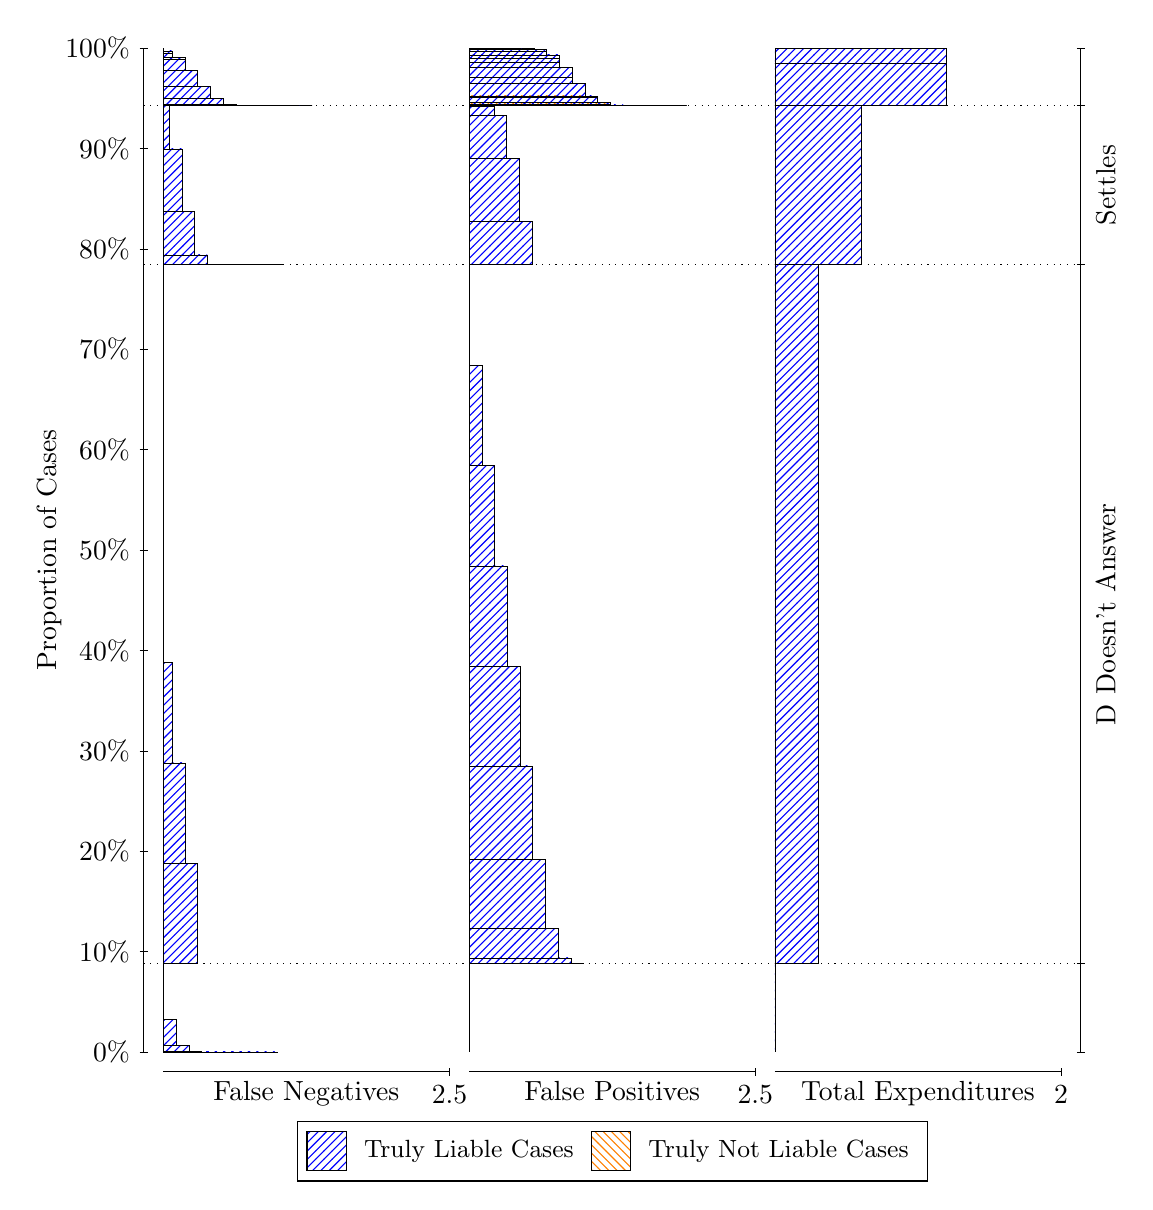
\begin{tikzpicture}
\draw[black, very thin] (1.5,1.75) -- (1.5,14.5);
\node[rotate=90, text=black, anchor=center] at (0.3, 8.125) {Proportion of Cases};
\draw[black, very thin] (1.45,1.75) -- (1.55,1.75);
\node[text=black, anchor=east] at (1.45, 1.75) {0\%};
\draw[black, very thin] (1.45,3.025) -- (1.55,3.025);
\node[text=black, anchor=east] at (1.45, 3.025) {10\%};
\draw[black, very thin] (1.45,4.3) -- (1.55,4.3);
\node[text=black, anchor=east] at (1.45, 4.3) {20\%};
\draw[black, very thin] (1.45,5.575) -- (1.55,5.575);
\node[text=black, anchor=east] at (1.45, 5.575) {30\%};
\draw[black, very thin] (1.45,6.85) -- (1.55,6.85);
\node[text=black, anchor=east] at (1.45, 6.85) {40\%};
\draw[black, very thin] (1.45,8.125) -- (1.55,8.125);
\node[text=black, anchor=east] at (1.45, 8.125) {50\%};
\draw[black, very thin] (1.45,9.4) -- (1.55,9.4);
\node[text=black, anchor=east] at (1.45, 9.4) {60\%};
\draw[black, very thin] (1.45,10.675) -- (1.55,10.675);
\node[text=black, anchor=east] at (1.45, 10.675) {70\%};
\draw[black, very thin] (1.45,11.95) -- (1.55,11.95);
\node[text=black, anchor=east] at (1.45, 11.95) {80\%};
\draw[black, very thin] (1.45,13.225) -- (1.55,13.225);
\node[text=black, anchor=east] at (1.45, 13.225) {90\%};
\draw[black, very thin] (1.45,14.5) -- (1.55,14.5);
\node[text=black, anchor=east] at (1.45, 14.5) {100\%};

\draw[black, very thin] (13.4,1.75) -- (13.4,14.5);
\draw[black, very thin] (13.35,1.75) -- (13.45,1.75);
\node[anchor=west] at (13.35, 1.75) {};
\draw[black, very thin] (13.35,2.872) -- (13.45,2.872);
\node[anchor=west] at (13.35, 2.872) {};
\draw[black, very thin] (13.35,11.749) -- (13.45,11.749);
\node[anchor=west] at (13.35, 11.749) {};
\draw[black, very thin] (13.35,13.771) -- (13.45,13.771);
\node[anchor=west] at (13.35, 13.771) {};
\draw[black, very thin] (13.35,14.5) -- (13.45,14.5);
\node[anchor=west] at (13.35, 14.5) {};

\draw[black, very thin, pattern color=blue, pattern=north east lines] (1.75,1.75) rectangle (3.2033,1.75);
\draw[black, very thin, pattern color=blue, pattern=north east lines] (1.75,1.75) rectangle (3.0419,1.75);
\draw[black, very thin, pattern color=blue, pattern=north east lines] (1.75,1.75) rectangle (2.8804,1.75);
\draw[black, very thin, pattern color=blue, pattern=north east lines] (1.75,1.75) rectangle (2.7189,1.75);
\draw[black, very thin, pattern color=blue, pattern=north east lines] (1.75,1.75) rectangle (2.5574,1.75);
\draw[black, very thin, pattern color=blue, pattern=north east lines] (1.75,1.75) rectangle (2.3959,1.7503);
\draw[black, very thin, pattern color=blue, pattern=north east lines] (1.75,1.7503) rectangle (2.2344,1.7579);
\draw[black, very thin, pattern color=blue, pattern=north east lines] (1.75,1.7579) rectangle (2.073,1.8357);
\draw[black, very thin, pattern color=blue, pattern=north east lines] (1.75,1.8357) rectangle (1.9115,2.1659);
\draw[black, very thin, pattern color=orange, pattern=north west lines] (1.75,2.1659) rectangle (1.75,2.1659);
\draw[black, very thin, pattern color=blue, pattern=north east lines] (1.75,2.1659) rectangle (1.75,2.872);
\draw[black, very thin, pattern color=blue, pattern=north east lines] (1.75,2.872) rectangle (2.186,4.147);
\draw[black, very thin, pattern color=blue, pattern=north east lines] (1.75,4.147) rectangle (2.0245,5.422);
\draw[black, very thin, pattern color=blue, pattern=north east lines] (1.75,5.422) rectangle (1.863,6.697);
\draw[black, very thin, pattern color=orange, pattern=north west lines] (1.75,6.697) rectangle (1.75,6.697);
\draw[black, very thin, pattern color=blue, pattern=north east lines] (1.75,6.697) rectangle (1.75,11.749);
\draw[black, very thin, pattern color=blue, pattern=north east lines] (1.75,11.749) rectangle (3.276,11.749);
\draw[black, very thin, pattern color=blue, pattern=north east lines] (1.75,11.749) rectangle (3.1145,11.749);
\draw[black, very thin, pattern color=blue, pattern=north east lines] (1.75,11.749) rectangle (2.953,11.749);
\draw[black, very thin, pattern color=blue, pattern=north east lines] (1.75,11.749) rectangle (2.7916,11.749);
\draw[black, very thin, pattern color=blue, pattern=north east lines] (1.75,11.749) rectangle (2.6301,11.749);
\draw[black, very thin, pattern color=blue, pattern=north east lines] (1.75,11.749) rectangle (2.4686,11.755);
\draw[black, very thin, pattern color=blue, pattern=north east lines] (1.75,11.755) rectangle (2.3071,11.874);
\draw[black, very thin, pattern color=blue, pattern=north east lines] (1.75,11.874) rectangle (2.1456,12.427);
\draw[black, very thin, pattern color=blue, pattern=north east lines] (1.75,12.427) rectangle (1.9841,13.219);
\draw[black, very thin, pattern color=blue, pattern=north east lines] (1.75,13.219) rectangle (1.8227,13.771);
\draw[black, very thin, pattern color=orange, pattern=north west lines] (1.75,13.771) rectangle (1.75,13.771);
\draw[black, very thin, pattern color=blue, pattern=north east lines] (1.75,13.771) rectangle (3.6393,13.771);
\draw[black, very thin, pattern color=blue, pattern=north east lines] (1.75,13.771) rectangle (3.4779,13.771);
\draw[black, very thin, pattern color=blue, pattern=north east lines] (1.75,13.771) rectangle (3.3164,13.771);
\draw[black, very thin, pattern color=blue, pattern=north east lines] (1.75,13.771) rectangle (3.1549,13.771);
\draw[black, very thin, pattern color=blue, pattern=north east lines] (1.75,13.771) rectangle (3.1549,13.771);
\draw[black, very thin, pattern color=blue, pattern=north east lines] (1.75,13.771) rectangle (2.9934,13.771);
\draw[black, very thin, pattern color=blue, pattern=north east lines] (1.75,13.771) rectangle (2.9934,13.771);
\draw[black, very thin, pattern color=blue, pattern=north east lines] (1.75,13.771) rectangle (2.8319,13.772);
\draw[black, very thin, pattern color=blue, pattern=north east lines] (1.75,13.772) rectangle (2.6704,13.786);
\draw[black, very thin, pattern color=blue, pattern=north east lines] (1.75,13.786) rectangle (2.509,13.787);
\draw[black, very thin, pattern color=blue, pattern=north east lines] (1.75,13.787) rectangle (2.509,13.858);
\draw[black, very thin, pattern color=blue, pattern=north east lines] (1.75,13.858) rectangle (2.3475,13.858);
\draw[black, very thin, pattern color=blue, pattern=north east lines] (1.75,13.858) rectangle (2.3475,13.86);
\draw[black, very thin, pattern color=blue, pattern=north east lines] (1.75,13.86) rectangle (2.3475,14.016);
\draw[black, very thin, pattern color=blue, pattern=north east lines] (1.75,14.016) rectangle (2.3475,14.016);
\draw[black, very thin, pattern color=blue, pattern=north east lines] (1.75,14.016) rectangle (2.186,14.016);
\draw[black, very thin, pattern color=blue, pattern=north east lines] (1.75,14.016) rectangle (2.186,14.216);
\draw[black, very thin, pattern color=blue, pattern=north east lines] (1.75,14.216) rectangle (2.0245,14.216);
\draw[black, very thin, pattern color=blue, pattern=north east lines] (1.75,14.216) rectangle (2.0245,14.218);
\draw[black, very thin, pattern color=blue, pattern=north east lines] (1.75,14.218) rectangle (2.0245,14.361);
\draw[black, very thin, pattern color=blue, pattern=north east lines] (1.75,14.361) rectangle (2.0245,14.378);
\draw[black, very thin, pattern color=blue, pattern=north east lines] (1.75,14.378) rectangle (1.863,14.378);
\draw[black, very thin, pattern color=blue, pattern=north east lines] (1.75,14.378) rectangle (1.863,14.433);
\draw[black, very thin, pattern color=blue, pattern=north east lines] (1.75,14.433) rectangle (1.863,14.463);
\draw[black, very thin, pattern color=orange, pattern=north west lines] (1.75,14.463) rectangle (1.75,14.463);
\draw[black, very thin, pattern color=blue, pattern=north east lines] (1.75,14.463) rectangle (1.75,14.5);
\draw[black, very thin, pattern color=orange, pattern=north west lines] (5.6333,1.75) rectangle (5.6333,1.75);
\draw[black, very thin, pattern color=blue, pattern=north east lines] (5.6333,1.75) rectangle (5.6333,2.872);
\draw[black, very thin, pattern color=orange, pattern=north west lines] (5.6333,2.872) rectangle (7.0867,2.872);
\draw[black, very thin, pattern color=blue, pattern=north east lines] (5.6333,2.872) rectangle (7.0867,2.8771);
\draw[black, very thin, pattern color=blue, pattern=north east lines] (5.6333,2.8771) rectangle (6.9252,2.9447);
\draw[black, very thin, pattern color=blue, pattern=north east lines] (5.6333,2.9447) rectangle (6.7637,3.3164);
\draw[black, very thin, pattern color=blue, pattern=north east lines] (5.6333,3.3164) rectangle (6.6022,4.193);
\draw[black, very thin, pattern color=blue, pattern=north east lines] (5.6333,4.193) rectangle (6.4407,5.3825);
\draw[black, very thin, pattern color=blue, pattern=north east lines] (5.6333,5.3825) rectangle (6.2793,6.6496);
\draw[black, very thin, pattern color=blue, pattern=north east lines] (5.6333,6.6496) rectangle (6.1178,7.9243);
\draw[black, very thin, pattern color=blue, pattern=north east lines] (5.6333,7.9243) rectangle (5.9563,9.1993);
\draw[black, very thin, pattern color=blue, pattern=north east lines] (5.6333,9.1993) rectangle (5.7948,10.474);
\draw[black, very thin, pattern color=blue, pattern=north east lines] (5.6333,10.474) rectangle (5.6333,11.749);
\draw[black, very thin, pattern color=orange, pattern=north west lines] (5.6333,11.749) rectangle (6.4327,11.749);
\draw[black, very thin, pattern color=blue, pattern=north east lines] (5.6333,11.749) rectangle (6.4327,12.302);
\draw[black, very thin, pattern color=blue, pattern=north east lines] (5.6333,12.302) rectangle (6.2712,13.094);
\draw[black, very thin, pattern color=blue, pattern=north east lines] (5.6333,13.094) rectangle (6.1097,13.647);
\draw[black, very thin, pattern color=blue, pattern=north east lines] (5.6333,13.647) rectangle (5.9482,13.766);
\draw[black, very thin, pattern color=blue, pattern=north east lines] (5.6333,13.766) rectangle (5.7867,13.771);
\draw[black, very thin, pattern color=blue, pattern=north east lines] (5.6333,13.771) rectangle (5.6333,13.771);
\draw[black, very thin, pattern color=orange, pattern=north west lines] (5.6333,13.771) rectangle (8.3947,13.771);
\draw[black, very thin, pattern color=blue, pattern=north east lines] (5.6333,13.771) rectangle (8.3947,13.771);
\draw[black, very thin, pattern color=orange, pattern=north west lines] (5.6333,13.771) rectangle (8.2332,13.771);
\draw[black, very thin, pattern color=blue, pattern=north east lines] (5.6333,13.771) rectangle (8.2332,13.771);
\draw[black, very thin, pattern color=orange, pattern=north west lines] (5.6333,13.771) rectangle (8.0717,13.771);
\draw[black, very thin, pattern color=blue, pattern=north east lines] (5.6333,13.771) rectangle (8.0717,13.771);
\draw[black, very thin, pattern color=blue, pattern=north east lines] (5.6333,13.771) rectangle (7.9102,13.771);
\draw[black, very thin, pattern color=orange, pattern=north west lines] (5.6333,13.771) rectangle (7.9102,13.771);
\draw[black, very thin, pattern color=blue, pattern=north east lines] (5.6333,13.771) rectangle (7.9102,13.771);
\draw[black, very thin, pattern color=orange, pattern=north west lines] (5.6333,13.771) rectangle (7.7487,13.771);
\draw[black, very thin, pattern color=blue, pattern=north east lines] (5.6333,13.771) rectangle (7.7487,13.772);
\draw[black, very thin, pattern color=blue, pattern=north east lines] (5.6333,13.772) rectangle (7.7487,13.772);
\draw[black, very thin, pattern color=orange, pattern=north west lines] (5.6333,13.772) rectangle (7.5873,13.772);
\draw[black, very thin, pattern color=blue, pattern=north east lines] (5.6333,13.772) rectangle (7.5873,13.776);
\draw[black, very thin, pattern color=blue, pattern=north east lines] (5.6333,13.776) rectangle (7.5873,13.779);
\draw[black, very thin, pattern color=blue, pattern=north east lines] (5.6333,13.779) rectangle (7.4258,13.79);
\draw[black, very thin, pattern color=orange, pattern=north west lines] (5.6333,13.79) rectangle (7.4258,13.79);
\draw[black, very thin, pattern color=blue, pattern=north east lines] (5.6333,13.79) rectangle (7.4258,13.808);
\draw[black, very thin, pattern color=orange, pattern=north west lines] (5.6333,13.808) rectangle (7.2643,13.808);
\draw[black, very thin, pattern color=blue, pattern=north east lines] (5.6333,13.808) rectangle (7.2643,13.872);
\draw[black, very thin, pattern color=blue, pattern=north east lines] (5.6333,13.872) rectangle (7.2643,13.893);
\draw[black, very thin, pattern color=orange, pattern=north west lines] (5.6333,13.893) rectangle (7.1028,13.893);
\draw[black, very thin, pattern color=blue, pattern=north east lines] (5.6333,13.893) rectangle (7.1028,14.053);
\draw[black, very thin, pattern color=blue, pattern=north east lines] (5.6333,14.053) rectangle (7.1028,14.055);
\draw[black, very thin, pattern color=blue, pattern=north east lines] (5.6333,14.055) rectangle (6.9413,14.13);
\draw[black, very thin, pattern color=orange, pattern=north west lines] (5.6333,14.13) rectangle (6.9413,14.13);
\draw[black, very thin, pattern color=blue, pattern=north east lines] (5.6333,14.13) rectangle (6.9413,14.255);
\draw[black, very thin, pattern color=blue, pattern=north east lines] (5.6333,14.255) rectangle (6.9413,14.255);
\draw[black, very thin, pattern color=blue, pattern=north east lines] (5.6333,14.255) rectangle (6.7799,14.313);
\draw[black, very thin, pattern color=blue, pattern=north east lines] (5.6333,14.313) rectangle (6.7799,14.374);
\draw[black, very thin, pattern color=blue, pattern=north east lines] (5.6333,14.374) rectangle (6.7799,14.414);
\draw[black, very thin, pattern color=blue, pattern=north east lines] (5.6333,14.414) rectangle (6.7799,14.414);
\draw[black, very thin, pattern color=blue, pattern=north east lines] (5.6333,14.414) rectangle (6.6184,14.453);
\draw[black, very thin, pattern color=blue, pattern=north east lines] (5.6333,14.453) rectangle (6.6184,14.485);
\draw[black, very thin, pattern color=blue, pattern=north east lines] (5.6333,14.485) rectangle (6.6184,14.485);
\draw[black, very thin, pattern color=blue, pattern=north east lines] (5.6333,14.485) rectangle (6.4569,14.499);
\draw[black, very thin, pattern color=blue, pattern=north east lines] (5.6333,14.499) rectangle (6.4569,14.499);
\draw[black, very thin, pattern color=blue, pattern=north east lines] (5.6333,14.499) rectangle (6.4569,14.499);
\draw[black, very thin, pattern color=blue, pattern=north east lines] (5.6333,14.499) rectangle (6.2954,14.499);
\draw[black, very thin, pattern color=blue, pattern=north east lines] (5.6333,14.499) rectangle (6.2954,14.5);
\draw[black, very thin, pattern color=blue, pattern=north east lines] (5.6333,14.5) rectangle (6.2954,14.5);
\draw[black, very thin, pattern color=blue, pattern=north east lines] (5.6333,14.5) rectangle (6.1339,14.5);
\draw[black, very thin, pattern color=blue, pattern=north east lines] (5.6333,14.5) rectangle (6.1339,14.5);
\draw[black, very thin, pattern color=blue, pattern=north east lines] (5.6333,14.5) rectangle (5.9724,14.5);
\draw[black, very thin, pattern color=blue, pattern=north east lines] (5.6333,14.5) rectangle (5.9724,14.5);
\draw[black, very thin, pattern color=blue, pattern=north east lines] (5.6333,14.5) rectangle (5.9724,14.5);
\draw[black, very thin, pattern color=blue, pattern=north east lines] (5.6333,14.5) rectangle (5.811,14.5);
\draw[black, very thin, pattern color=blue, pattern=north east lines] (5.6333,14.5) rectangle (5.811,14.5);
\draw[black, very thin, pattern color=blue, pattern=north east lines] (5.6333,14.5) rectangle (5.6495,14.5);
\draw[black, very thin, pattern color=blue, pattern=north east lines] (5.6333,14.5) rectangle (5.6333,14.5);
\draw[black, very thin, pattern color=orange, pattern=north west lines] (9.5167,1.75) rectangle (9.5167,1.75);
\draw[black, very thin, pattern color=blue, pattern=north east lines] (9.5167,1.75) rectangle (9.5167,2.872);
\draw[black, very thin, pattern color=orange, pattern=north west lines] (9.5167,2.872) rectangle (10.062,2.872);
\draw[black, very thin, pattern color=blue, pattern=north east lines] (9.5167,2.872) rectangle (10.062,11.749);
\draw[black, very thin, pattern color=orange, pattern=north west lines] (9.5167,11.749) rectangle (10.607,11.749);
\draw[black, very thin, pattern color=blue, pattern=north east lines] (9.5167,11.749) rectangle (10.607,13.771);
\draw[black, very thin, pattern color=orange, pattern=north west lines] (9.5167,13.771) rectangle (11.697,13.771);
\draw[black, very thin, pattern color=blue, pattern=north east lines] (9.5167,13.771) rectangle (11.697,14.308);
\draw[black, very thin, pattern color=orange, pattern=north west lines] (9.5167,14.308) rectangle (11.697,14.308);
\draw[black, very thin, pattern color=blue, pattern=north east lines] (9.5167,14.308) rectangle (11.697,14.5);
\draw[black, dotted] (1.5,2.872) -- (13.4,2.872);
\draw[black, dotted] (1.5,11.749) -- (13.4,11.749);
\draw[black, dotted] (1.5,13.771) -- (13.4,13.771);
\draw[black, very thin] (1.75,1.5) -- (5.3833,1.5);
\node[text=black, anchor=north] at (3.5667, 1.5) {False Negatives};
\draw[black, very thin] (5.3833,1.45) -- (5.3833,1.55);
\node[text=black, anchor=north] at (5.3833, 1.45) {2.5};

\draw[black, very thin] (5.6333,1.5) -- (9.2667,1.5);
\node[text=black, anchor=north] at (7.45, 1.5) {False Positives};
\draw[black, very thin] (9.2667,1.45) -- (9.2667,1.55);
\node[text=black, anchor=north] at (9.2667, 1.45) {2.5};

\draw[black, very thin] (9.5167,1.5) -- (13.15,1.5);
\node[text=black, anchor=north] at (11.333, 1.5) {Total Expenditures};
\draw[black, very thin] (13.15,1.45) -- (13.15,1.55);
\node[text=black, anchor=north] at (13.15, 1.45) {2};


\node[text=black, centered, rotate=90] at (13.72, 7.3107) {D Doesn't Answer};
\node[text=black, centered, rotate=90] at (13.72, 12.76) {Settles};


\draw (7.449999999999999,1.5) node[draw=none] (baseCoordinate) {};
\begin{scope}[align=center]
        \matrix[scale=0.5, draw=black, below=0.5cm of baseCoordinate, nodes={draw}, column sep=0.1cm]{
            \node[rectangle, draw, minimum width=0.5cm, minimum height=0.5cm, pattern color=blue, pattern=north east lines] {}; &
            \node[draw=none, font=\small, text=black] (B) {Truly Liable Cases}; &
            \node[rectangle, draw, minimum width=0.5cm, minimum height=0.5cm, pattern color=orange, pattern=north west lines] {}; &
            \node[draw=none, font=\small, text=black] (B) {Truly Not Liable Cases}; \\
            };
\end{scope}

\end{tikzpicture}
\end{document}